\chapter{Visão geral do projeto}
    
    O projeto basicamente consite no desenvolvimento de pesquisas e soluções de baixo custo para um sistema de 
    resfriamento do sensor Kistler tipo 6061BS utilizado no motor de foguete híbrido do LPQ da 
    Universidade de Brasília, visando respeitar os parâmetros de funcionamento do motor e do sensor.
    A realização do projeto consiste de uma equipe de 36 graduandos em diversas Engenharias, sendo que
    essa equipe se sub-dividiu em equipes menores baseadas em funções específicas, tais como: Controle, Processamento
    de dados, Estrutura, Gerência de Projeto e Transmissão de Calor.

\section{Propostas de Soluções}

    Após a realização de um curto período de estudos e pesquisas, nós identificamos três principais
    soluções para o problema de arrefecimento do sensor Kistler. Abaixo está uma tabela ilustrando as
    soluções e suas características baseado no modelo existente do sistema de arrefecimento da Kistler.

    \begin{table}[!htb]
        \centering
        \begin{tabular}{p{5cm}p{10cm}}
          \toprule
          \textbf{Hipótese 1}  &     Um sistema de distribuição baseado no original, 
                                    porém com um modelo de resfriador próprio do grupo.                             \\ \midrule
          \textbf{Hipótese 2} &     Um sistema baseado no original, 
                                    porém com um modelo de resfriador e líquido condutor do próprio grupo.   \\ \midrule
          \textbf{Hipótese 3} &     Um sistema totalmente novo.                      \\
          \bottomrule
        \end{tabular}
        \caption{Propostas de Soluções}
      \end{table}

\section{Estrutura Analítica do Projeto (EAP)}

\begin{figure}[!htb]
    \centering
    \includegraphics[width=17cm, height=10cm, keepaspectratio=true]{figuras/eap/EAP.eps}
    \caption{Estrutura Analítica do Projeto - EAP Geral}
 \end{figure}

 \begin{figure}[!htb]
    \centering
    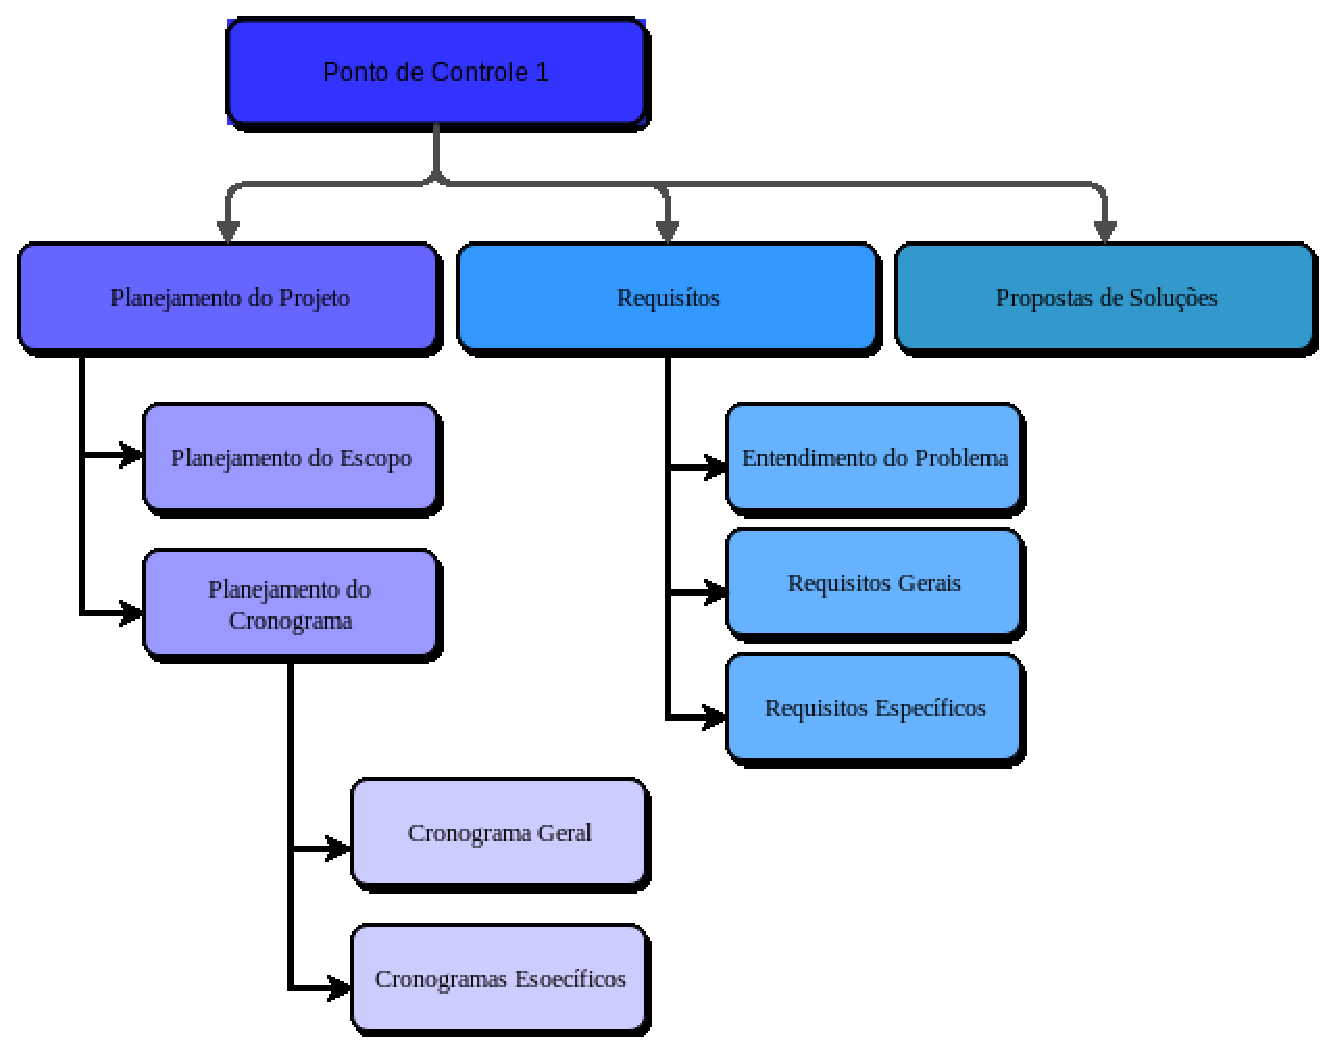
\includegraphics[width=11cm, height=10cm, keepaspectratio=true]{figuras/eap/EAP_1.eps}
    \caption{EAP - PC1}
 \end{figure}

 \begin{figure}[!htb]
    \centering
    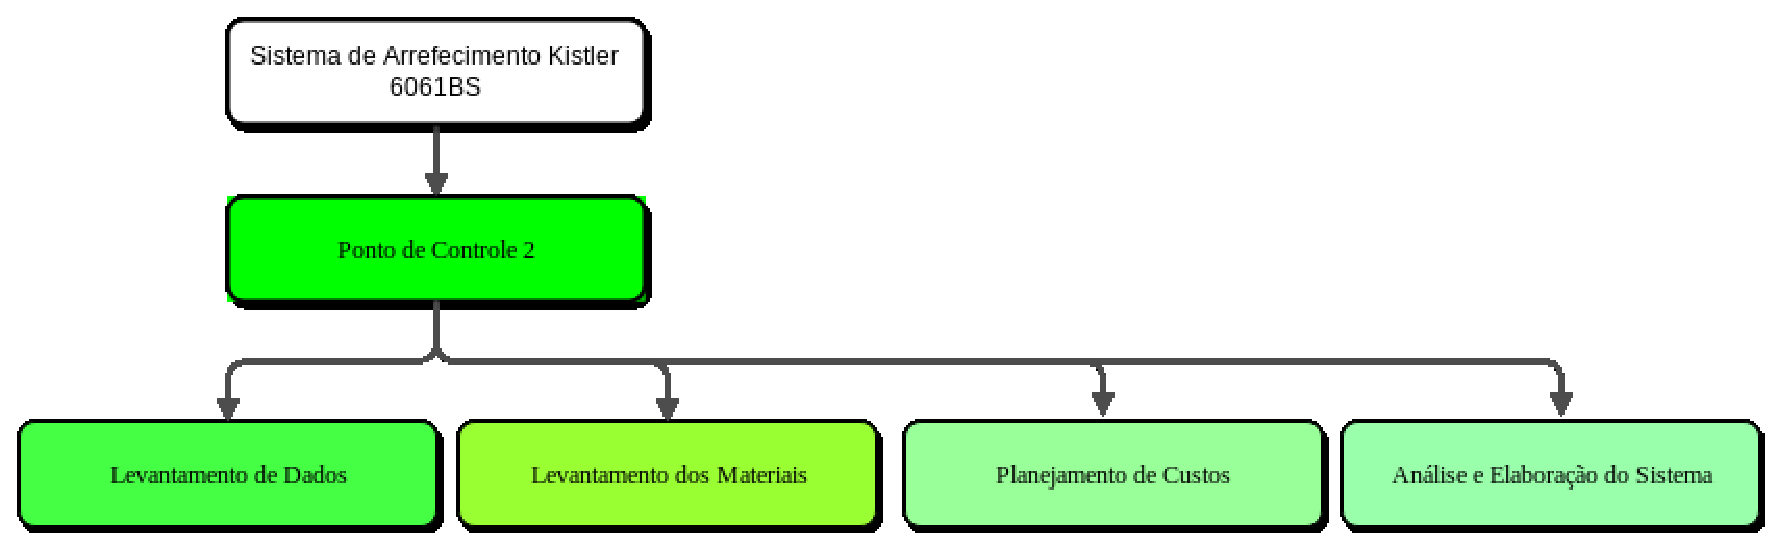
\includegraphics[width=17cm, height=15cm, keepaspectratio=true]{figuras/eap/EAP_2.eps}
    \caption{EAP - PC2}
 \end{figure}

 \begin{figure}[!htb]
    \centering
    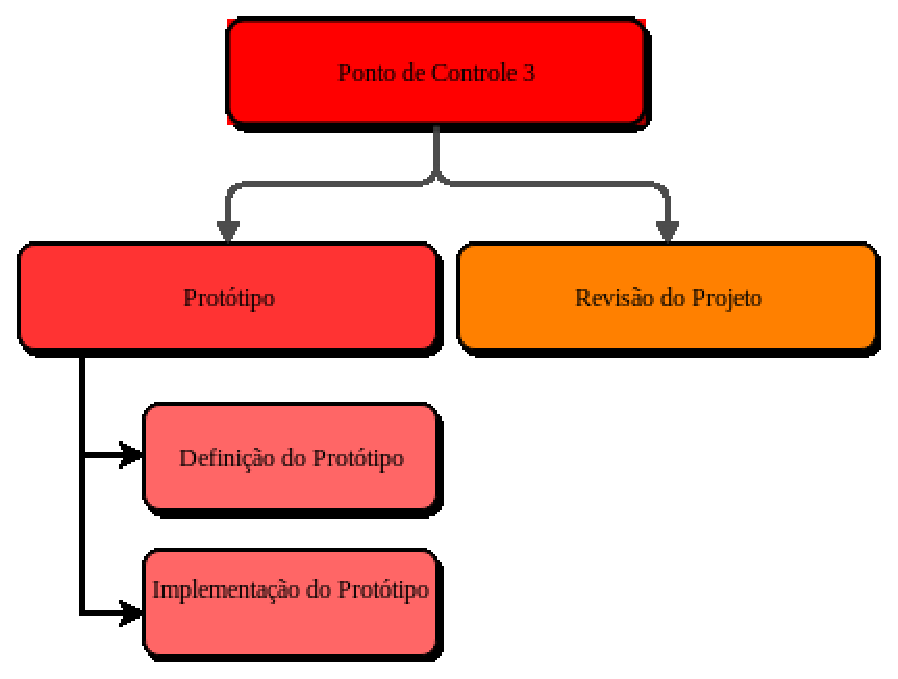
\includegraphics[width=9cm, height=8cm, keepaspectratio=true]{figuras/eap/EAP_3.eps}
    \caption{EAP - PC3}
 \end{figure}